\section{Introducing Objects}
\label{Sec: Introducing Objects}

In simulating real-world phenomena, it is essential to incorporate geometric shapes into the simulation environment to represent physical boundaries and objects accurately. The complexity of these shapes can vary significantly depending on the specific problem at hand, and selecting the appropriate coordinate system plays a critical role in simplifying the implementation. However, for ease of integration, a cartesian coordinate system is used throughout the simulations outlined in this report. While the general procedure of implementing geometric shapes in the simulation remains the same, this section exemplifies the process by focusing on two specific three-dimensional shapes. The first is a sphere, which is geometrically defined by its center vector and radius. To simulate the interaction between charged particles and the sphere, all grid nodes located within the sphere are assigned a fixed electric potential. This can be implemented in the simulation using the following approach:

\begin{figure}[H]
    \centering
    \begin{lstlisting}
def add_sphere(self, x0, radius, phi_sphere):
    self.sphere_x0 = Vec3(*x0)  # Save sphere centroid
    self.sphere_rad2 = radius * radius  # Save radius squared
    
    # Loop over all nodes
    for i in range(self.ni):
        for j in range(self.nj):
            for k in range(self.nk):
                x = self.pos(i, j, k)  # Node position
                if self.in_sphere(x):
                    self.objectid.data[i, j, k] = 1  # Set object flag
                    self.phi.data[i, j, k] = phi_sphere  # Set potential

def in_sphere(self, x):
    """Check if a point x is inside the sphere."""
    return (x-self.sphere_x0).dot(x-self.sphere_x0) <= self.sphere_rad2
\end{lstlisting}
    \caption{Caption}
    \label{fig:enter-label}
\end{figure}

The basic procedure involves iterating over all nodes in the system and checking whether each point lies within the desired geometry. If this condition is met, the node is assigned a specific object value, allowing for the storage of information about the simulation world for further analysis in tools such as ParaView. An illustration of such a charged sphere is shown below:

\begin{figure}
    \centering
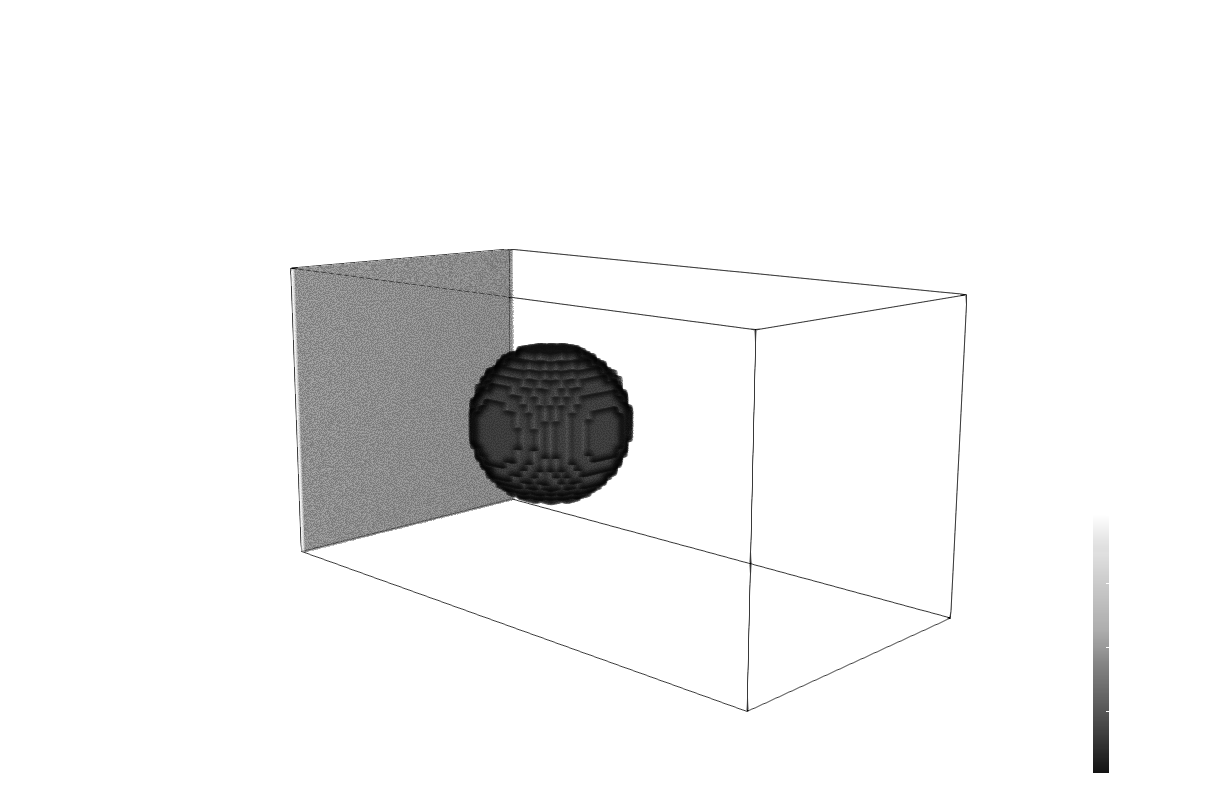
\includegraphics[width=0.7\linewidth]{figures/sphere_paraview.png}    
    \caption{Caption}
    \label{fig:enter-label}
\end{figure}




\begin{figure} [H]
    \centering
    \begin{lstlisting}
def add_plane_with_hole(self, z_0, thickness, phi_plane, hole_0,hole_r):

# Loop over all nodes
for i in range(self.ni):
    for j in range(self.nj):
        for k in range(self.nk):
            x, y, z = self.pos(i, j, k)  # coordinates of the current node
            
            # Calculate the distance from the hole-center in the XY plane
            xy_dist2 = (x - hole_0[0]) ** 2 + (y - hole_0[1]) ** 2
            
            # Check if the current node is within the plane thickness
            # and outside the circular hole area
            if z_0 <= z < (z_0 + thickness) and xy_dist2 > hole_radius2:
                self.objectid.data[i, j, k] = 1  # Set object flag
                self.phi.data[i, j, k] = phi_plane  # Set potential
    \end{lstlisting}
    \caption{Caption}
    \label{fig:enter-label}
\end{figure}
